
\begin{figure*}[htpb]
    \centering
    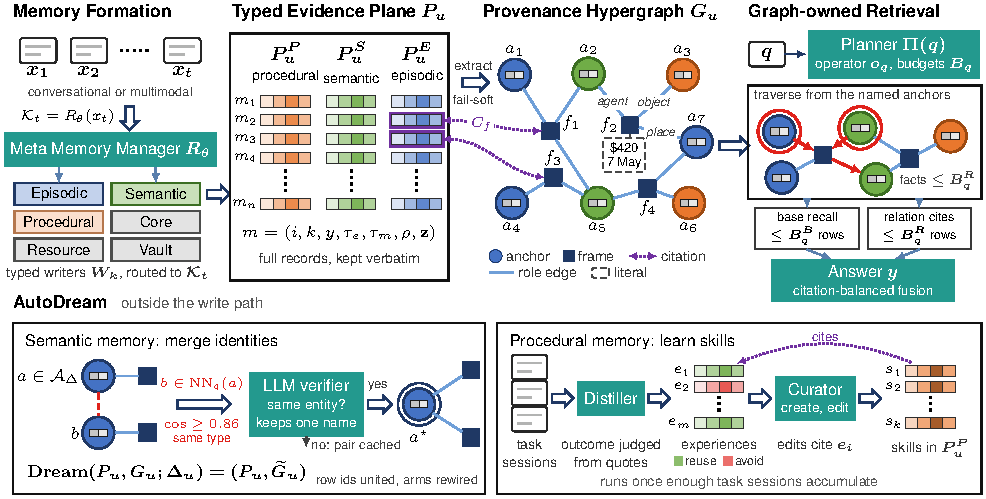
\includegraphics[width=\textwidth]{figures/mirix_fig1_v2.pdf}
    \caption{Overview of \ours. Typed writers fill the evidence plane $P_u$, the provenance
    hypergraph $G_u$ indexes it with n-ary frames that cite their sources, retrieval traverses
    $G_u$ under explicit budgets, and AutoDream consolidates outside the write path.}
    \label{fig:mirix-overview}
\end{figure*}



\section{Introduction}



Large language model (LLM) agents now work over horizons far longer than a
single context window~\citep{luo2025agentsurvey,agentmemorysurvey}. A personal
agent accumulates months of conversation with its user, and a task agent meets
similar problems across many episodes. Memory lets such agents carry
information across sessions~\citep{lscs}, so that they can personalize their
responses~\citep{zhang2026personaagent}, stay consistent with what they were
told~\citep{memgpt,mem0}, and reuse what worked
before~\citep{wang2025awm,xia2026skillrl}. Benchmarks now measure this
ability on long conversations~\citep{locomo,longmemeval}, long
documents~\citep{memoryagentbench}, multi-session agentic
tasks~\citep{he2026memoryarena}, and lifelong
personalization~\citep{memorycd}.

Benchmarks score a memory by its answers, but a team that deploys one asks more
of it. A memory that agents can rely on in practice has to meet three
requirements at once. It has to be accurate about the particulars of past
experience, such as a name, a date, a count, or the distinction between two
events, and about the connections between them. It has to be practical, which
means deployable with the models a team already uses, nothing to train, answers
that can be traced to stored records, and consolidation that cannot destroy what
was stored. It also has to be efficient, with answer latency and token cost per
question that stay bounded as the history grows. 
% Existing systems give up one of
% the three. Systems that consolidate records into extracted facts or
% abstractions~\citep{mem0,ye2026autodreamer} are compact, but the details they
% drop are gone for good, and consolidation can make a memory faulty even when it
% is distilled from useful experience~\citep{zhang2026faultymemories}. Graph
% memories organize the same content around entities and their
% relations~\citep{zep,edge2024graphrag}, yet binary triples split an n-ary fact
% into fragments~\citep{luo2025hypergraphrag,hypermem}.
% Systems that keep every record lose nothing, but they leave retrieval to search
% an ever larger and noisier history~\citep{agentmemorysurvey}. Parametric
% memories store experience in model weights or latent
% states~\citep{memoryllm,mplus,self-param,behrouz2024titans}, which requires
% training and rules out closed models.

Each family of existing systems gives up at least one of the three. Systems
that consolidate records into extracted facts or
abstractions~\citep{mem0,ye2026autodreamer} are compact but give up accuracy:
the details they discard are gone for good, and consolidation can make a
memory faulty even when it is distilled from useful
experience~\citep{zhang2026faultymemories}. Systems that keep every record and
retrieve from them directly lose nothing but give up efficiency, since
retrieval must search an ever larger and noisier
history~\citep{agentmemorysurvey}. Graph memories organize the same content
around entities and their relations~\citep{zep,edge2024graphrag}, but binary
triples split an n-ary fact into fragments and lose the connections among its
participants~\citep{luo2025hypergraphrag}. Hypergraph
memories~\citep{hypermem} group episodes under topics and facts under
episodes, but their hyperedges record which unit belongs where rather than
the participants of a fact, and retrieval descends from topic summaries
written at storage time, so a detail is reachable only after its topic has
been retrieved. File-system memories, such as the auto memory of Claude
Code~\citep{claudecodememory}, route retrieval through summaries in the same way: they keep notes in plain
files behind a size-capped index that is loaded into every session, and the
agent opens a file on the strength of its one-line summary. A detail that no
summary mentions is reachable only by string search, which neither resolves
an entity across files nor follows its relations, and index entries past the
cap are not loaded at the start of a session. Both families prune top down to
bound their cost, and both pay for the pruning with recall on details their
summaries do not reflect. Parametric memories store experience in model
weights or latent states~\citep{memoryllm,mplus,self-param,behrouz2024titans}
and give up practicality, since they require training and rule out closed
models.


The requirements also weigh differently for the two uses of memory. Recent
studies separate user-centric memory, which personalizes an agent to its user,
from agent-centric memory, which accumulates the agent's own experience, and
they find that the two face reversed
challenges~\citep{agentmemorysurvey,harnessmemory}. A user-centric memory has
to record a user's history broadly and connect its pieces, because a later
question may depend on any detail of that history~\citep{memorycd,ma2026memaudit}.
An agent-centric memory has to be precise and refined instead. It distills
trajectories into strategies and
skills~\citep{zhao2024expel,ouyang2026reasoningbank,xia2026metaclaw}, and
retrieving too much can pull the agent's attention away from the context that
matters for its next action~\citep{harnessmemory}. A practical system has to
serve both uses from one store.
\Cref{fig:mirix-user-centric,fig:mirix-agent-centric} trace one example of each
setting through \ours.

\begin{figure}[!t]
    \centering
    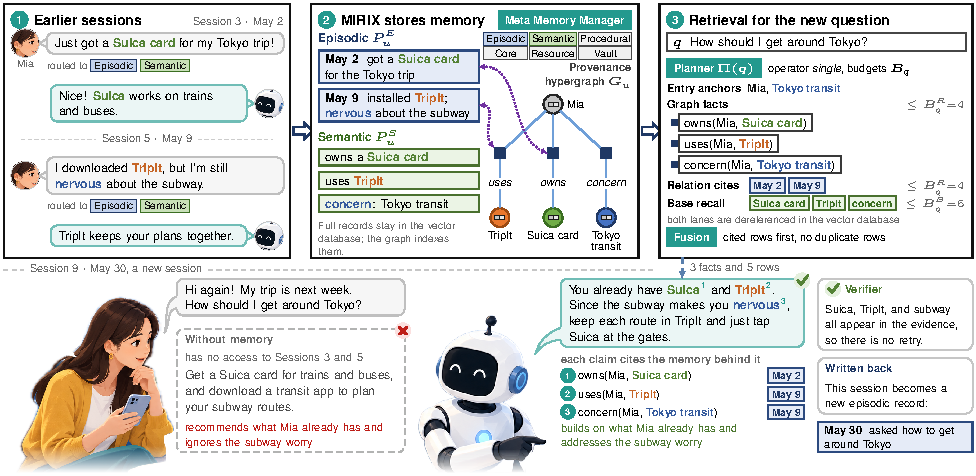
\includegraphics[width=\linewidth]{figures/mirix_user_centric.pdf}
    \caption{User-centric memory. Sessions are stored as episodic and semantic records, and a
    later question retrieves graph facts with their source rows to give a personalized answer.}
    \label{fig:mirix-user-centric}
\end{figure}

In this work, we present \ours, a multi-agent memory system designed to be
practical, accurate, and efficient at once. It keeps the multi-agent design of
MIRIX~\citep{mirix} and rethinks how memory is stored, indexed, retrieved, and
consolidated so that a specific layer meets each requirement
(\Cref{fig:mirix-overview}). Six memory agents under a Meta Memory Manager write
complete records to a \emph{typed evidence plane} in a vector database, the system
of record, so details survive consolidation and every graph fact the answer
receives cites the rows it came from. The graph is only an index. The database write commits first, a failed graph write never rolls back a stored memory, and
a failed graph read falls back to direct evidence retrieval. A
\emph{provenance hypergraph} indexes the entities, events, relations, roles, and
times in episodic and semantic records as n-ary frames that cite the rows they
were extracted from and carry dates, prices, and counts as literals, and undated
events with similar wording keep distinct identities. At query time, a
deterministic planner sets explicit budgets, retrieval enters the hypergraph at the anchors that match the question, and the answer receives graph facts together
with the records they cite (\Cref{sec:retrieval}). The evidence a question inspects is therefore bounded by construction
and does not grow with the length of the history.

Like sleep-time and offline consolidation
methods~\citep{lin2025sleeptime,ye2026autodreamer}, AutoDream consolidates
memory outside the write path, and it treats the two kinds of memory in
opposite ways. For semantic memory, it consolidates identities and never
rewrites evidence. It pairs each anchor introduced by new semantic rows with its
nearest anchors of the same identity-stable type, such as a person or a place,
and asks a language model whether a pair denotes one entity. A confirmed merge
unites the citations of the two anchors and rewires the frames that mention
them, while event anchors, fact frames, and stored records stay unchanged, so a
merge can never destroy a stored memory. Its cost depends on the newly written
semantic frontier rather than on the total size of memory, verification runs
under explicit pair caps, and negative decisions are cached so that later cycles
do not pay for the same pair again. For procedural memory, AutoDream refines
instead. It judges each finished task session from quotes in its transcript,
distills lessons worth reusing and mistakes worth avoiding, and lets a
curator~\citep{zhang2026ace} create or edit skills whose edits can cite the
experiences behind them.

We evaluate \ours on conversational memory, long-document question answering,
personalized generation, and procedural memory for interactive agents. \ours
has the highest accuracy of all compared memory systems on both conversational
benchmarks, 91.4\% on LoCoMo in our runs and 72.6\% on LongMemEval-S, 14.3 points
above the strongest baseline. On LoCoMo, the hypergraph raises accuracy over flat
memory from 85.7\% to 88.4\%, with the largest gain on multi-hop questions, and
AutoDream raises every question type and lifts the overall score to 91.4\%. On
LongMemEval-S, the hypergraph alone adds 11.2 points. On the single-hop and multi-hop document QA tasks of
MemoryAgentBench~\citep{memoryagentbench}, with AutoDream disabled, it answers
83.0\% and 71.0\% of the questions, 31.0 and 22.0 points above the strongest
baseline, and on MemoryCD~\citep{memorycd} it has the highest value on all four
metrics for cross-domain review summarization. Used as procedural memory, \ours
gives the highest mean success among the compared memory methods on
ALFWorld~\citep{shridhar2021alfworld}, at 76.4\% with GPT-6 Luna against 73.6\%
for Agent Workflow Memory (AWM)~\citep{wang2025awm} and 69.4\% without memory, and on WebShop~\citep{yao2022webshop}, at
37.4\%. With GPT-5.2 it reaches 49.2\% accuracy on
MetaClaw-Bench~\citep{xia2026metaclaw}, against 44.0\% reported for the MetaClaw
skill library.

What makes these results usable is the cost at which they come. With AutoDream
disabled, \ours answers faster than HyperMem, the strongest baseline, on all five
benchmarks we timed, ingests the two conversational benchmarks in less time, and
uses fewer answer tokens on four of the five. As procedural memory, on WebShop it
uses the fewest training and test tokens among the memory methods while reaching
the highest success. The cost is paid when long documents are ingested. Building the graph makes
their ingestion about four times slower than flat memory and slower than that
baseline. The full system with AutoDream is not timed, and the retrieval bounds
cover the evidence a question inspects, not latency measured as the history
grows. No model is fine-tuned, the same system runs with closed and open
models, and the code is public.

Our contributions are as follows.
\begin{itemize}[leftmargin=*,nosep]
    \item \textbf{Accurate and practical.} A layered memory design in which six
    typed memory agents keep complete records as the system of record and a
    provenance-preserving n-ary hypergraph serves only as their index, with
    occurrence identities that keep distinct events apart and fail-soft
    indexing that never rolls back a stored memory.
    \item \textbf{One memory for users and agents.} To the best of our
    knowledge, \ours is the first memory system that handles both user-centric
    and agent-centric memory, serving personalization and the refinement of
    agent skills from one store.
    \item \textbf{Efficient and safe to consolidate.} Graph-owned retrieval runs
    under explicit budgets and returns graph facts together with the records
    that justify them. AutoDream merges duplicate entity anchors under explicit
    caps without touching stored memories, which adds 3.0 points on LoCoMo, and
    distills task sessions into skills for procedural memory.
\end{itemize}
The rest of the paper is organized as follows. \Cref{sec:method} presents
\ours. It states the problem and the three technical requirements, introduces
the typed evidence plane and the provenance hypergraph that indexes it,
describes graph-owned retrieval under explicit budgets, and explains how
AutoDream consolidates semantic and procedural memory outside the write path.
\Cref{sec:experiments} evaluates the accuracy of \ours on conversational recall,
long-document question answering, and personalized generation, its use as
agent memory on ALFWorld, WebShop, and MetaClaw-Bench, and its cost in
ingestion time, answer latency, and tokens. \Cref{sec:related} relates \ours to
prior work on memory systems for LLM agents, multi-agent systems, and memory
consolidation, and \Cref{sec:conclusion} concludes and discusses the
limitations of this study. \Cref{app:method} gives the details of the method,
and \Cref{app:results} gives the full results behind the figures.


\begin{figure}[!t]
    \centering
    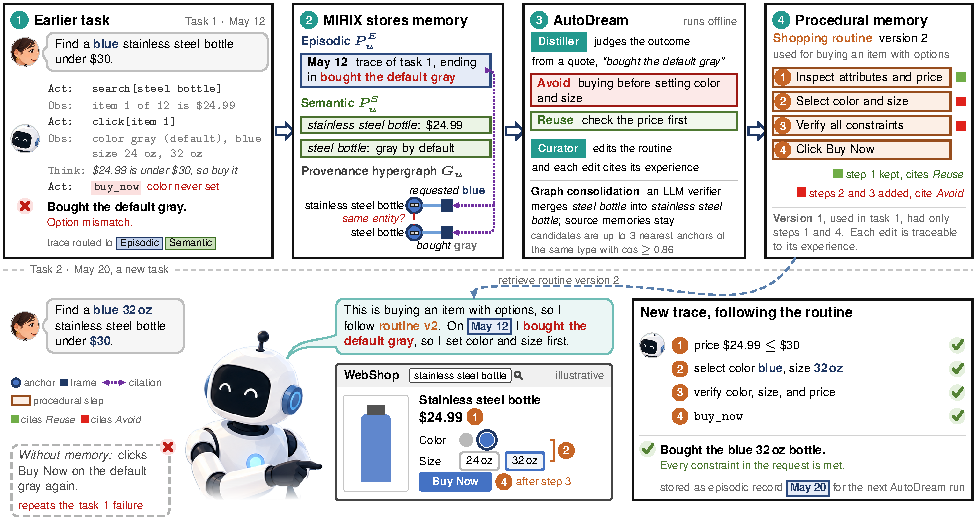
\includegraphics[width=\linewidth]{figures/mirix_agent_centric.pdf}
    \caption{Agent-centric memory. AutoDream turns a failed purchase into experiences and a
    revised routine, which a later task follows to meet every constraint.}
    \label{fig:mirix-agent-centric}
\end{figure}
